\chapter{Ultraviolette Divergenzen und ihre Beseitigung durch Supersymmetrie}

\lectureoverview{Bevor wir die formale Mathematik der Supersymmetrie einführen, sollten wir das Problem, das sie lösen soll, genau beschreiben. Wir betrachten ultraviolette Divergenzen sowohl im Orts- als auch im Impulsraum, leiten das Kurzstreckenverhalten skalarer und fermionischer Propagatoren mithilfe der Dimensionsanalyse her und schätzen die führenden Schleifenkorrekturen zur Masse eines Skalars ab. Eine skalare Schleife und eine Fermionschleife weisen dieselbe quadratische Abhängigkeit vom Cutoff, jedoch entgegengesetzte Vorzeichen auf. Supersymmetrie wird dann überzeugend, wenn wir fragen, welches Prinzip ihre Kopplungen, Multiplizitäten und Massen so aufeinander abstimmen könnte, dass die Aufhebung strukturell und nicht zufällig ist.}

\section{Warum kehren wir zu den Divergenzen zurück?}

Der Plan war, sofort mit dem mathematischen Apparat der Supersymmetrie zu beginnen. Es ist jedoch besser, die Abstraktion um eine Vorlesung aufzuschieben und die Motivation neu aufzubauen. Die frühere Darstellung der Divergenzen und der Massenrenormierung ging schnell voran. Ohne zunächst genau zu erkennen, was behoben werden muss, wirkt die Supersymmetrie wie eine willkürliche mathematische Erfindung.

Feynman-Diagramme spielen in der Teilchenphysik auf zwei eng miteinander verbundenen Gebieten eine Rolle. Am bekanntesten ist ihre Verwendung zur Ordnung von Streuamplituden. Wir legen ein- und auslaufende Teilchen fest und summieren die Amplituden aller Diagramme der erforderlichen Ordnung. Außerdem dienen sie zur Konstruktion einer \emph{effektiven Lagrange-Dichte}. Das Wort ``effektiv'' ist hier kein Lob im Sinne von ungewöhnlich erfolgreich. Es bedeutet, dass die Beschreibung näherungsweise gilt: Unzugängliche Details auf kurzen Distanzen wurden eliminiert oder herausintegriert, und ihr Einfluss ist in den verbleibenden Parametern und Wechselwirkungen enthalten.

Jede solche Beschreibung gilt nur in einem bestimmten Bereich. Diesen können wir durch eine kleinste verlässliche Distanz angeben, hier bezeichnet mit \(\delta\), oder durch einen größten verlässlichen Impuls,
\begin{equation}
\Lambda\sim \delta^{-1}.
\end{equation}
Die beiden Cutoffs sind keine voneinander unabhängigen Annahmen. Sie sind Fourier-duale Beschreibungen derselben ultravioletten Grenze.

\section{Ein Propagator, zwei Beschreibungen}

Der Propagator ist die Amplitude dafür, ein Teilchen an einem Raumzeitpunkt zu erzeugen oder einzusetzen und es an einem anderen zu entfernen oder nachzuweisen. Seien die beiden Punkte \(x^\mu\) und \(y^\mu\), und bezeichnen wir ihren Abstand mit
\begin{equation}
\Delta^\mu=y^\mu-x^\mu.
\end{equation}
Das Kleinbuchstabensymbol \(\delta\) verwenden wir für den Cutoff, damit er nicht mit dem Abstand verwechselt wird.

Translationsinvarianz bedeutet, dass ein freier Propagator von \(x\) und \(y\) nur über \(\Delta\) abhängt. Dasselbe Objekt lässt sich fouriertransformieren:
\begin{equation}
G(\Delta)
=\int\frac{d^4k}{(2\pi)^4}\,e^{-ik\cdot\Delta}\,\widetilde G(k).
\end{equation}

Auf die Frage ``Was sind die Fourier-konjugierten Größen des Orts?'' lautet die Antwort aus dem Hörsaal: der Impuls. Daher entspricht die Beschreibung einer Schleife im Ortsraum als Propagator, der zu seinem Ausgangspunkt zurückkehrt, der Beschreibung im Impulsraum als Integral über alle Impulse, die um die Schleife laufen können. Die Rechenregeln im Impulsraum verlangen, an jedem Vertex die Impulserhaltung durchzusetzen; für die vorliegende Abschätzung der Potenzen macht der Ortsraum die Argumentation transparenter.

Diese Äquivalenz macht das Ultraviolettproblem sichtbar, noch bevor wir etwas berechnen. Im Ortsraum untersucht eine Schleife den Grenzfall zusammenfallender Punkte \(\Delta\to0\). Im Impulsraum untersucht sie den Grenzfall \(|k|\to\infty\). Große Impulse bedeuten kurze Wellenlängen; eine Singularität bei kurzen Distanzen und eine Divergenz bei hohen Impulsen sind also dasselbe Phänomen in unterschiedlichen Koordinaten.

In der Vorlesung geht es um die einfachsten Spin-Klassen: Skalarfelder, Fermionfelder und, im Hintergrund, Eichfelder. Skalare haben Spin null und werden durch ein einkomponentiges Feld \(\phi(x)\) dargestellt. Als die Vorlesung 2010 aufgezeichnet wurde, war das Higgs noch nicht entdeckt; es wurde als das wichtigste in der Teilchenphysik erwartete Skalarteilchen beschrieben. Dieser historische Kontext erklärt die scherzhafte Bezeichnung ``higgly-wiggly'': Das Feld war physikalisch dringend von Interesse, aber experimentell noch nicht bestätigt.

Für ein reelles Skalarfeld lässt sich der Propagator schematisch schreiben als
\begin{equation}
G_\phi(x,y)=\expect{0|T\!\left\{\phi(x)\phi(y)\right\}|0}
=G_\phi(\Delta).
\end{equation}
Die Zeitordnungs-Konvention und die Normierung spielen für unsere Potenzzählung keine Rolle. Entscheidend ist, dass die beiden Feldeinsetzungen die Erzeugung an einem Punkt und die Vernichtung am anderen beschreiben.

\begin{classroomqa}
\audiencequestion{Sind \(x\) und \(y\) Orte im Raum oder in der Raumzeit? \lecturetimestamp{00:09:31}}
\lecturerresponse{Es sind Raumzeitpunkte. Jeder davon ist ein Vierervektor. Der Propagator hängt daher von ihrem vierdimensionalen Abstand und, in einem Lorentz-invarianten Vakuum, vom entsprechenden invarianten Intervall ab.}
\end{classroomqa}

Ein Teilchen mit Spin ein Halb wird durch ein Dirac-Feld \(\psi_i(x)\) beschrieben. Der Index \(i\) ist ein Spinorindex, keine räumliche Komponente; deshalb ist der Propagator eine Matrix:
\begin{equation}
S_{ij}(x,y)=\expect{0|T\!\left\{\psi_i(x)\bar\psi_j(y)\right\}|0}
=S_{ij}(\Delta).
\end{equation}

Eine Frage an den Hörsaal liefert die Anzahl der Komponenten: Ein Dirac-Feld in vier Dimensionen hat vier komplexe Komponenten. Ein masseloses Weyl-Feld lässt sich mit zwei komplexen Komponenten beschreiben, sodass linkshändige und rechtshändige Felder getrennt behandelt werden können. Für die vorliegende Dimensionsanalyse zählt allein, dass der Propagator eine Spinormatrixstruktur hat.

Da \(S_{ij}\) eine \(4\times4\)-Matrix ist, lässt sie sich nach den Dirac-Matrizen entwickeln. Zunächst lassen wir diese Indizes weg und führen sie wieder ein, sobald sie benötigt werden. Damit behaupten wir nicht, dass die Matrixstruktur fehlt; wir vereinfachen die Darstellung bewusst, während wir das ultraviolette Potenzgesetz herleiten.

\begin{classroomqa}
\audiencequestion{Wann muss in einem Propagator das konjugierte oder adjungierte Feld auftreten? \lecturetimestamp{00:14:06}}
\lecturerresponse{Bei einem reellen, neutralen Skalarfeld in dieser schematischen Betrachtung enthält dasselbe Feld Erzeugungs- und Vernichtungsoperatoren, sodass kein separates adjungiertes Feld nötig ist. Bei einem geladenen Feld müssen Teilchen- und Antiteilchenoperatoren unterschieden werden. Daher spielen \(\psi\), \(\psi^\dagger\) und kovariant \(\bar\psi=\psi^\dagger\gamma^0\) für ein Elektron unterschiedliche Rollen.}
\end{classroomqa}

Das physikalische Higgs-Teilchen ist neutral, obwohl das zugrunde liegende Higgs-Feld des Standardmodells ein elektroschwaches Dublett ist. In der Vorlesung dient das reelle neutrale Skalarfeld als einfaches Modell; für die Abschätzung im Ultravioletten genügt diese Vereinfachung.\editorialnote{Diese Unterscheidung verhindert, dass das schematische Beispiel eines reellen Skalarfelds für eine vollständige Aussage über das elektroschwache Higgs-Multiplett gehalten wird.}

\section{Natürliche Einheiten und die Dimension eines Skalarfelds}

Wir setzen \(\hbar=c=1\). Damit haben Länge und Zeit dieselbe Einheit, während Energie, Masse und Impuls die Einheit der inversen Länge haben:
\begin{equation}
[m]=[E]=[p]=L^{-1}.
\end{equation}
Die Wirkung tritt in der Phase \(e^{iS}\) auf und ist daher dimensionslos. Eine typische Wirkung für ein Skalarfeld in vier Raumzeitdimensionen lautet
\begin{equation}
S_\phi=\int d^4x\left[
\frac12\partial_\mu\phi\,\partial^\mu\phi
-\frac12m^2\phi^2
-\frac{\lambda}{4!}\phi^4
+\cdots\right].
\end{equation}
Die üblichen Faktoren \(1/2\) und \(1/4!\) beeinflussen die Dimensionsanalyse nicht.

Wir beginnen mit dem kinetischen Term. Da \([d^4x]=L^4\) und \([\partial_\mu]=L^{-1}\), folgt aus der Dimensionslosigkeit
\begin{align}
1
&=L^4\left(L^{-1}[\phi]\right)^2,\\
[\phi]&=L^{-1}.
\end{align}
Der Massenterm dient als Überprüfung:
\begin{equation}
L^4[m^2][\phi^2]
=L^4L^{-2}L^{-2}=1.
\end{equation}

Die nächste Frage an den Hörsaal betrifft die Dimension der quartischen Kopplung. Sie ist in vier Raumzeitdimensionen dimensionslos:
\begin{equation}
L^4[\lambda][\phi]^4=L^4[\lambda]L^{-4}=1
\quad\Longrightarrow\quad [\lambda]=L^0.
\end{equation}
Damit ist die Wechselwirkung \(\phi^4\) in vier Dimensionen besonders. Die Dimensionen von \(\phi^6\) und höheren Wechselwirkungen folgen nach derselben Regel, doch ihre Kopplungen enthalten negative Potenzen der Masse und weisen damit auf eine stärker eingeschränkte Rolle in der effektiven Theorie hin.

Die Felddimensionen zeigen also bereits, welche Wechselwirkungen mit dimensionslosen Koeffizienten auftreten können. Dieselbe Methode bestimmt sowohl die Propagatoren als auch die Yukawa-Kopplung, ohne dass wir ein detailliertes Feynman-Integral auswerten müssen.

\section{Der skalare Propagator bei kurzen Distanzen}

Betrachten wir zunächst ein masseloses Skalarfeld. Es gibt keine intrinsische Längenskala, daher ist nur der Abstand \(\Delta\) als Skala verfügbar. Translationsinvarianz lässt lediglich \(\Delta\) übrig, Lorentz-Invarianz reduziert die Abhängigkeit auf dessen invarianten Betrag, und das Produkt zweier Skalarfelder hat die Dimension \(L^{-2}\). Bis auf einen numerischen Faktor gilt
\begin{equation}
G_0(\Delta)\sim\frac{1}{\Delta^2}.
\end{equation}
Faktoren wie \(4\pi^2\) lassen sich allein aus Dimensionsgründen nicht bestimmen.

Eine Masse führt die Compton-Wellenlänge \(m^{-1}\) ein. Ihre Wirkung lässt sich am einfachsten anhand der Dispersionsrelation verstehen:
\begin{equation}
E=\sqrt{\bm p^{,2}+m^2},
\qquad
E=|\bm p|\quad(m=0).
\end{equation}
Für \(|\bm p|\gg m\) ist die Masse vernachlässigbar. Da hohe Impulse kurze Distanzen untersuchen, muss der massive Propagator für \(\Delta\to0\) gegen das masselose Verhalten \(1/\Delta^2\) gehen. Bei Distanzen, die viel größer als \(m^{-1}\) sind, wird die Propagation unterdrückt. Die Vorlesung stellt diesen Sachverhalt schematisch dar durch
\begin{equation}
G_m(\Delta)\sim \frac{e^{-m|\Delta|}}{\Delta^2}.
\end{equation}
Dies ist ausdrücklich keine exakte Formel. In vierdimensionalem euklidischem Raum ist der exakte freie Propagator proportional zu \(mK_1(mr)/r\), wobei \(r=|\Delta|\) gilt; er weist dieselbe ultraviolette Singularität \(1/r^2\) und einen exponentiellen Abfall bei großen Distanzen mit einem Potenzgesetz als Vorfaktor auf.\editorialnote{Die Besselfunktion liefert die übliche präzise Ergänzung zum schematischen Exponentialterm der Vorlesung und wird für die Potenzzählung nicht benötigt.}

Die entscheidende Aussage ist einfach: Die Masse schwächt die Propagation über große Distanzen ab, behebt aber nicht die Singularität bei zusammenfallenden Punkten. In hinreichender Nähe eines Punktes wird jede endliche Masse irrelevant.

\section{Das skalare Tadpole-Diagramm und die Feinabstimmung}

Die quartische Wechselwirkung \(\lambda\phi^4\) erzeugt einen Vertex mit vier Linien. Wir verbinden zwei seiner Beine miteinander und lassen zwei externe skalare Beine übrig. Das resultierende Tadpole-Diagramm korrigiert den Koeffizienten von \(\phi^2\) und damit das Quadrat der Skalarmasse.

Das erhaltene Bild zeigt genau den Übergang von der Dimensionsanalyse zu dieser Schleifenkorrektur. Links ist weiterhin die Dispersionsrelation zu sehen, rechts sind noch Teile der skalaren Wirkung und der Felddimension erkennbar, und in der Mitte ist gerade das kleine Tadpole-Diagramm hinzugekommen.

\begin{figure}[H]
\centering
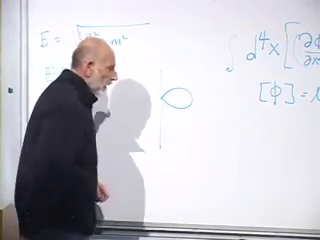
\includegraphics[width=0.72\textwidth]{lecture_03_figure_02.png}
\lectureframe{00:28:30.560}

\medskip
\begin{tikzpicture}[line width=0.8pt,scale=1.0]
  \draw[dashed] (-2.6,0) -- (0,0) -- (2.6,0);
  \fill (0,0) circle (0.055);
  \draw (0,0) .. controls (-0.85,0.7) and (-0.85,1.6) .. (0,1.6)
                .. controls (0.85,1.6) and (0.85,0.7) .. (0,0);
\end{tikzpicture}
\caption{Die Tafel beim Übergang zur skalaren Selbstenergie, gefolgt von einer zurückhaltenden schematischen Neuzeichnung der Tadpole-Topologie. Der Screenshot zeigt eindeutig die Schleife, die relativistische und die masselose Energieformel sowie einen Teil der Wirkung; verdeckte Koeffizienten und Bezeichnungen werden nicht als sichtbar ausgegeben.}
\end{figure}

Am Vertex kann das Skalarteilchen absorbiert und wieder emittiert werden, während die beiden anderen Beine vom Punkt fortlaufen und zu ihm zurückkehren. Bis auf numerische und kombinatorische Faktoren beträgt die Korrektur
\begin{equation}
\delta m_\phi^2\sim \lambda G_\phi(0).
\end{equation}
Der Propagator am Koinzidenzpunkt ist in der Kontinuumsnäherung unendlich. Eine effektive Theorie beansprucht keine Gültigkeit bei beliebig kleinen Distanzen; daher setzen wir \(|\Delta|\geq\delta\). Dann gilt
\begin{equation}
G_\phi(0)\longrightarrow G_\phi(\delta)sim\frac{1}{\delta^2},
\qquad
\delta m_\phi^2\sim\frac{\lambda}{\delta^2}sim\lambda\Lambda^2.
\end{equation}
Man nennt die Divergenz quadratisch, weil sie zwei Potenzen des Impuls-Cutoffs enthält. Die Integration im Impulsraum führt zum selben Ergebnis: Ein übermäßiger Beitrag stammt von beliebig großen Schleifenimpulsen. Ob die kürzeste Skala letztlich durch die große Vereinheitlichung, die Quantengravitation oder etwas noch Unvorstelltes festgelegt wird, ändert nichts an dieser Diagnose der effektiven Theorie.

Dies ist ein Feinabstimmungsproblem. Wenn \(\delta\) extrem klein und \(\lambda\) nicht außerordentlich winzig ist, ist die Strahlungskorrektur viel größer als das bei niedrigen Energien beobachtete Quadrat der Skalarmasse. Der nackte Koeffizient und die Schleifenkorrektur müssen sich dann bis auf eine unplausibel große Zahl von Stellen aufheben:
\begin{equation}
m_{\mathrm{physical}}^2
=m_{\mathrm{bare}}^2+\delta m_\phi^2.
\end{equation}
Der massive Propagator rettet die Situation nicht. Bei den für die Divergenz verantwortlichen Distanzen gilt \(e^{-m|\Delta|}\simeq1\). Die ultraviolette Schleife hat die Masse längst vergessen, bevor sie den Cutoff erreicht.

\section{Dimensionen von Fermionen und ihr Propagator}

Nun wiederholen wir dieselbe Dimensionsanalyse für ein Dirac-Fermion. Seine freie Wirkung lautet
\begin{equation}
S_\psi=\int d^4x\,
\bar\psi\left(i\gamma^\mu\partial_\mu-m\right)\psi.
\end{equation}
Die Gamma-Matrizen sind numerisch und dimensionslos. Der kinetische Term enthält nur eine Ableitung, also gilt
\begin{align}
1
&=L^4[\bar\psi]L^{-1}[\psi],\\
[\psi]=[\bar\psi]&=L^{-3/2}.
\end{align}
Halbzahlige Potenzen sollten nicht beunruhigen; Fermionen bringen an vielen Stellen Faktoren von ein Halb mit sich.

\begin{classroomqa}
\audiencequestion{Wäre es nicht einfacher, \([\psi]\) aus dem Massenterm herzuleiten? \lecturetimestamp{00:36:02}}
\lecturerresponse{Ja. Der Massenterm ergibt \(L^4L^{-1}[\bar\psi\psi]=1\), also \([\bar\psi\psi]=L^{-3}\) und \([\psi]=L^{-3/2}\). Zuerst wurde die Herleitung aus dem kinetischen Term verwendet, weil sie auch in der masselosen Theorie sinnvoll bleibt und zeigt, warum die Fermionmasse als \(m\) und nicht als \(m^2\) auftritt.}
\end{classroomqa}

Zwei Fermionfelder haben zusammen die Dimension \(L^{-3}\); daher lautet die kompakte Dimensionsabschätzung der Vorlesung für den masselosen Propagator
\begin{equation}
S(\Delta)\sim\frac{1}{|\Delta|^3}.
\end{equation}
Mit wiederhergestellter Matrixstruktur erhält man den präziseren, durch Lorentz-Kovarianz erforderlichen Zähler:
\begin{equation}
S_{ij}(\Delta)
\propto
\frac{\left(\gamma_\mu\Delta^\mu\right)_{ij}}
{\left(\Delta^2\right)^2}.
\end{equation}
Der Zähler liefert eine zusätzliche Potenz der Länge, der Nenner enthält daher vier Potenzen des Intervalls; die Gesamtdimension bleibt \(L^{-3}\). Wie beim Skalar unterdrückt eine Fermionmasse den Propagator bei großen Abständen, ändert aber nicht dessen Skalierung bei kurzen Distanzen.

\section{Warum eine geschlossene Fermionschleife ein negatives Vorzeichen hat}

Nun können wir fragen, ob ein fermionisches Diagramm die problematische bosonische Selbstenergie aufheben könnte. Das skalare Tadpole-Diagramm hat bis auf positive numerische Faktoren, etwa Potenzen von \(\pi\), und kombinatorische Koeffizienten ein positives Vorzeichen. Eine geschlossene Fermionschleife trägt das entgegengesetzte Vorzeichen.

\begin{classroomqa}
\audiencequestion{Hängt das Minuszeichen der Fermionschleife mit der früheren Diskussion einer vollen Drehung zusammen? \lecturetimestamp{00:40:21}}
\lecturerresponse{Es gehört zur selben fermionischen Vorzeichenstruktur. Der hier nützliche Beweis beruht jedoch auf der Antisymmetrie beim Vertauschen und nicht auf der geometrischen Orientierung einer Schleife. Wir schneiden zwei Schleifen auf, vertauschen die identischen Teilchen und verbinden die Linien wieder. Durch die Vertauschung werden aus zwei Schleifen eine; nur bei Fermionen kommt dabei ein Minuszeichen hinzu.}
\end{classroomqa}

Das Argument verdient eine ausführliche Darstellung. Angenommen, ein Einschleifendiagramm hat das Vorzeichen \(\sigma\), also plus oder minus. Zwei voneinander getrennte, identische Schleifen haben dann das Vorzeichen
\begin{equation}
\sigma^2=+1.
\end{equation}
Schneiden wir beide Schleifen gleichzeitig auf, so laufen nun zwei identische Teilchen zwischen den Schnittstellen. Ihre gewöhnliche Zweiteilchen-Wellenfunktion ist für Bosonen symmetrisch und für Fermionen antisymmetrisch:
\begin{align}
\Psi_B(x_1,x_2)&=+\Psi_B(x_2,x_1),\\
\Psi_F(x_1,x_2)&=-\Psi_F(x_2,x_1).
\end{align}
Die Antisymmetrie erklärt auch das Pauli-Prinzip: Befinden sich beide Fermionen im selben Zustand, ändert der Austausch physikalisch nichts, muss aber das Vorzeichen der Wellenfunktion umkehren; folglich muss sie verschwinden.

Wir verbinden die aufgeschnittenen Linien wieder, nachdem wir die beiden Teilchen vertauscht haben. Topologisch sind aus den zwei Schleifen eine geworden. Die Amplitude der beiden nicht vertauschten Schleifen war positiv. Durch den Austausch bleibt sie für Bosonen positiv, kehrt sich aber für Fermionen um. Daher gilt
\begin{equation}
\begin{aligned}
\operatorname{sign}(\text{closed boson loop})&=+1,\\
\operatorname{sign}(\text{closed fermion loop})&=-1.
\end{aligned}
\end{equation}
Dieses Ergebnis ist allgemein: Jede unabhängige geschlossene Fermionschleife liefert einen Faktor \(-1\).

\section{Die Yukawa-Schleife}

Kehren wir zur Skalarmasse zurück. Ein Boson kann nicht in ein einzelnes Fermion übergehen, da sich dabei die Fermionzahlparität ändern würde. Die einfachste fermionische Korrektur entsteht, wenn sich das Skalarfeld in ein Fermion-Antifermion-Paar aufspaltet, das eine Schleife durchläuft und wieder rekombiniert. Die Wechselwirkung ist eine Yukawa-Kopplung,
\begin{equation}
\mathcal L_Y=-g\phi\bar\psi\psi.
\end{equation}
Beim Higgs können die Fermionen Quarks oder Leptonen sein. Es gibt zwei Wechselwirkungspunkte und damit zwei Faktoren \(g\).

Beim skalaren Tadpole-Diagramm gab es einen Punkt; seine Gesamtposition konnte festgelegt werden, da die Translationsinvarianz lediglich das Raumzeitvolumen liefert. Die Yukawa-Schleife hat zwei Punkte. Wir können einen Punkt oder äquivalent ihre mittlere Position festlegen, müssen aber über ihren relativen Abstand \(\Delta\) integrieren. Jeder Fermionpropagator liefert den Kurzstreckenfaktor \(1/|\Delta|^3\), also
\begin{equation}
\delta m_{\phi,F}^2
\sim
-g^2\int_{|\Delta|\geq\delta}d^4\Delta\,
\frac{1}{|\Delta|^6}.
\end{equation}

Nachdem die beiden Propagatoren, das Integral über den Abstand und die beiden Kopplungen hingeschrieben sind, wird noch ein letzter Faktor aus dem Hörsaal erfragt. Die Antwort lautet: das Minuszeichen. Die beiden Propagatoren schließen sich zu einer Fermionschleife, sodass das gesamte ansonsten positive Kurzstreckenintegral mit \(-1\) multipliziert wird.

Die Divergenz lässt sich bereits durch Dimensionsanalyse bestimmen. \(d^4\Delta\) liefert vier Längenpotenzen, im Nenner treten sechs auf, und als einzige verbleibende Längenskala bleibt der Cutoff:
\begin{equation}
\int_{|\Delta|\geq\delta}
\frac{d^4\Delta}{|\Delta|^6}
\sim\frac{1}{\delta^2}.
\end{equation}
In vierdimensionalen euklidischen Polarkoordinaten lässt sich dies explizit zeigen:
\begin{equation}
\int_{\delta}^{R}d^4\Delta\,\frac{1}{|\Delta|^6}
=2\pi^2\int_{\delta}^{R}dr\,\frac{r^3}{r^6}
=\pi^2\left(\frac{1}{\delta^2}-\frac{1}{R^2}\right).
\end{equation}
Spinorspuren und Propagatornormierungen verändern den Koeffizienten, nicht aber die quadratische Potenz des Cutoffs.\editorialnote{Das Radialintegral ist eine übliche explizite Form der in der Vorlesung vorgenommenen Dimensionsabschätzung. Es ist in euklidischem Abstand geschrieben, wo die Positivität und die ultraviolette Potenzzählung unmittelbar zu erkennen sind.}

\begin{classroomqa}
\audiencequestion{Kann eine Umkehrung oder Wahl der Integrationsgrenzen das Vorzeichen ändern? \lecturetimestamp{00:51:06}}
\lecturerresponse{Nein. Dies ist kein eindimensionales orientiertes Integral, dessen Grenzen das physikalische Vorzeichen festlegen. Es handelt sich um ein Integral über vier Komponenten oder, noch übersichtlicher, über ein positives Radialmaß. Sein ultravioletter Betrag ist positiv. Der negative Beitrag stammt ausschließlich von der geschlossenen Fermionschleife.}
\end{classroomqa}

\begin{classroomqa}
\audiencequestion{Welche Dimension hat die Yukawa-Kopplung \(g\)? \lecturetimestamp{00:51:51}}
\lecturerresponse{Sie ist in vier Dimensionen dimensionslos. Da \([\phi]=L^{-1}\) und \([\bar\psi\psi]=L^{-3}\), hat das Produkt \(\phi\bar\psi\psi\) die Dimension \(L^{-4}\), die durch \(d^4x\) genau ausgeglichen wird.}
\end{classroomqa}

Die führende fermionische Korrektur lautet daher
\begin{equation}
\delta m_{\phi,F}^2
\sim -C_F\frac{g^2}{\delta^2}
=-C_Fg^2\Lambda^2,
\end{equation}
wobei \(C_F>0\) numerische Faktoren sowie Spin- und Multiplizitätsfaktoren enthält. Der skalare Schleifenbeitrag hat die entsprechende Form
\begin{equation}
\delta m_{\phi,B}^2
\sim+C_B\frac{\lambda}{\delta^2}
=+C_B\lambda\Lambda^2.
\end{equation}
Das Feinabstimmungsproblem haben wir noch nicht gelöst, aber etwas Unverzichtbares gefunden: einen Beitrag mit demselben Grad der ultravioletten Divergenz und entgegengesetztem Vorzeichen.

\section{Was für die Aufhebung erforderlich ist}

Es wäre ein außerordentlicher Zufall, wenn voneinander unabhängige Kopplungen gerade die Relation
\begin{equation}
C_B\lambda=C_Fg^2
\end{equation}
erfüllen würden, und zwar genau genug für eine große Hierarchie von Skalen. Die Vorlesung fasst dies als \(g^2=\lambda\) zusammen und lässt dabei konventionsabhängige Faktoren und Multiplizitäten weg. Eine echte Lösung erfordert eine mathematische Struktur, die diese Relation erzwingt, statt sie lediglich zuzulassen.

Das ist die Motivation für die Supersymmetrie. Sie bringt Bosonen und Fermionen miteinander in Beziehung und beschränkt ihre Kopplungen auf Kombinationen, bei denen sich viele ansonsten problematische divergente Terme aufheben. Diese Aufhebung wiederholt sich dann über verschiedene Diagramme hinweg, weil sie aus einer Symmetrie folgt und nicht daraus, dass die Parameter für jede Schleife einzeln angepasst wurden.

Auch der Abgleich der Massen ist wichtig. Sind die Massen von Bosonen und Fermionen identisch, lassen sich ihre vollständigen Propagatoren am besten paarweise einander zuordnen. Unterscheiden sich die Massen geringfügig, heben sich die vollständigen endlichen Ergebnisse nicht exakt auf, da die Propagatoren bei Distanzen vergleichbar mit ihren Compton-Wellenlängen voneinander abweichen. Ihre gemeinsame Kurzstreckenasymptotik kann jedoch den divergenten Anteil aufheben:
\begin{equation}
\mathcal I_B(\Delta)-\mathcal I_F(\Delta)
\quad\hbox{may be finite as}\quad \Delta\to0,
\end{equation}
wobei \(\mathcal I_B\) und \(\mathcal I_F\) die vollständigen bosonischen beziehungsweise fermionischen Schleifenintegranden nach Einbeziehung der Vertizes, Zähler und Multiplizitäten bezeichnen. Die Propagatoren selbst haben unterschiedliche Dimensionen und werden nicht direkt voneinander abgezogen. Selbst wenn sich die ultravioletten Terme aufheben, kann ein endlicher Rest bleiben. Hier setzt die Möglichkeit einer näherungsweisen oder gebrochenen Supersymmetrie an. Exakte Gleichheit ergibt die klarste Aufhebung; eine hinreichend kontrollierte Brechung kann die ultraviolette Katastrophe dennoch beseitigen und zugleich beobachtbare Massensaufspaltungen zulassen.

Damit sind wir bei der Supersymmetrie angelangt, ohne ihre Algebra bereits angeschrieben zu haben. Die Argumentationskette ist vollständig:
\begin{equation}
\begin{gathered}
G_\phi(\Delta)\sim \Delta^{-2},
\qquad
\delta m_{\phi,B}^2\sim+C_B\lambda\Lambda^2,\\[0.4em]
S_\psi(\Delta)\sim \Delta^{-3},
\qquad
\delta m_{\phi,F}^2\sim-C_Fg^2\Lambda^2,\\[0.4em]
\text{symmetry-enforced matching}\\
\Longrightarrow\quad
\text{quadratic divergences cancel}.
\end{gathered}
\end{equation}
Als Nächstes müssen wir das abstrakte Symmetrieprinzip verstehen, das diese Relationen erzwingt, und konkrete Beispiele für seine Wirkung betrachten.